\documentclass[border=3pt,tikz]{standalone}
\usetikzlibrary{arrows}
\usetikzlibrary{positioning}
\usetikzlibrary{calc}
\usetikzlibrary{arrows}
\begin{document}
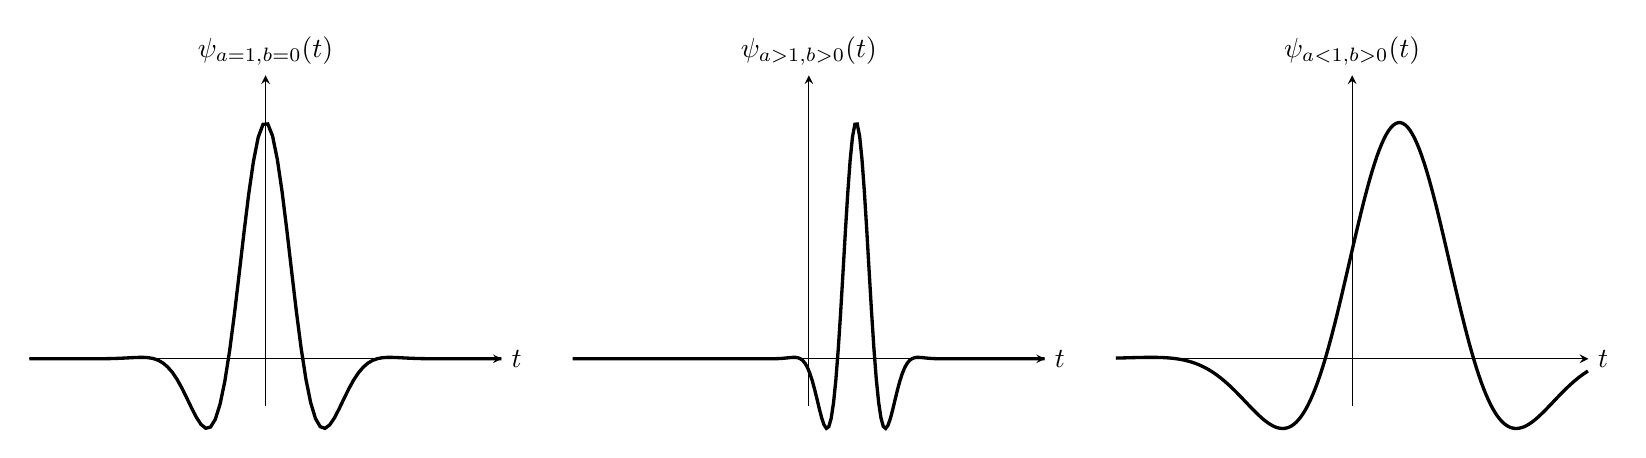
\begin{tikzpicture}[samples = 200, scale=3]

    \draw[-{stealth}] (-1, 0) -- (1,0) node[right] {$t$};
    \draw[-{stealth}] (0,-0.2) -- (0,1.2) node[above] {$\psi_{a=1, b=0}(t)$};
    \draw[color=black, very thick, domain=-1:1, samples=100, variable = \t]   plot ({\t}, {exp(-(4*\t)^2) * cos(\t*180/pi*10)});
    
    
    \begin{scope}[xshift=2.3cm] 
    
    \draw[-{stealth}] (-1, 0) -- (1,0) node[right] {$t$};
    \draw[-{stealth}] (0,-0.2) -- (0,1.2) node[above] {$\psi_{a>1, b>0} (t)$};
    
    \draw[color=black, very thick, domain=-1:1, samples=200, variable = \t]   plot ({\t}, {exp(-(8*(\t-0.2))^2) * cos(2*(\t-0.2)*180/pi*10)});
    
    \end{scope}
    
    \begin{scope}[xshift=4.6cm] 
    
    \draw[-{stealth}] (-1, 0) -- (1,0) node[right] {$t$};
    \draw[-{stealth}] (0,-0.2) -- (0,1.2) node[above] {$\psi_{a<1, b>0}(t)$};
    
    \draw[color=black, very thick, domain=-1:1, samples=200, variable = \t]   plot ({\t}, {exp(-(2*(\t-0.2))^2) * cos(0.5*(\t-0.2)*180/pi*10)});
    
    \end{scope}
    
    
    \end{tikzpicture}
\end{document}